\documentclass{article}
\usepackage{hyperref, url, graphicx, xcolor}
\newcommand{\uicontrol}[1]{\textcolor{blue}{\textbf{#1}}}
\begin{document}
%https://www.xmlmind.com/tutorials/DITA/index.html#task_element
\section*{Installing GNU Emacs}
\begin{description}
	\item[Prerequities] Windows NT 4.0 or any subsequent version of Windows. 5Mb of free
	disk space.
\end{description}
\begin{enumerate}
	\item Unzip the distribution anywhere.
	\item We recommend to use the free, open source, \href{http://www.info-zip.org/}{Info-ZIP}
	utility to do so.
	\begin{verbatim}
		C:\> unzip emacs-21.3-bin-i386.zip
	\end{verbatim}
	\begin{itemize}
		\item Doing this will create an \path{emacs-21.3} directory.
	\end{itemize}
	\item Go to the bin subdirectory \verb|C:> cd emacs-21.3\bin|
	\item Run addpm.
	\begin{verbatim}
		C:\emacs-21.3\bin> addpm
	\end{verbatim}
	\begin{itemize}
		\item A confirmation dialog box is displayed.\\
		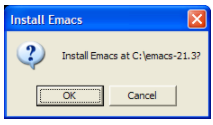
\includegraphics{confirm-install-emacs}
	\end{itemize}
	\item Click \uicontrol{OK} to confirm.
\end{enumerate}
\end{document}
